\documentclass[conference,compsoc]{IEEEtran}
\IEEEoverridecommandlockouts
\ifCLASSOPTIONcompsoc
  \usepackage[nocompress]{cite}
\else
  \usepackage{cite}
\fi
\usepackage{amsmath,amssymb,amsfonts}
\usepackage{graphicx}
\usepackage{textcomp}
\usepackage{xcolor}
\usepackage{booktabs}
\usepackage{placeins}
\def\BibTeX{{\rm B\kern-.05em{\sc i\kern-.025em b}\kern-.08em
    T\kern-.1667em\lower.7ex\hbox{E}\kern-.125emX}}

\makeatletter
\newcommand{\linebreakand}{%
  \end{@IEEEauthorhalign}
  \hfill\mbox{}\par
  \mbox{}\hfill\begin{@IEEEauthorhalign}
}
\makeatother

\begin{document}

\title{Deep Learning-Based MRI-to-DTI Synthesis for Inferring White Matter Connectivity from Structural Scans\\
}

\author{
\IEEEauthorblockN{Purav N Khincha}
\IEEEauthorblockA{\textit{Department of Computer}\\
\textit{Science and Engineering}\\
\textit{PES University}\\
Bangalore, India \\
puravkhincha@gmail.com}
\and
\IEEEauthorblockN{Pranavi Sistla}
\IEEEauthorblockA{\textit{Department of Computer}\\
\textit{Science and Engineering}\\
\textit{PES University}\\
Bangalore, India \\
pranavi.sistla9526@gmail.com}
\and
\IEEEauthorblockN{Mahitha G}
\IEEEauthorblockA{\textit{Department of Computer}\\
\textit{Science and Engineering}\\
\textit{PES University}\\
Bangalore, India \\
mahithag@pes.edu}
}

\maketitle

\begin{abstract}
Diffusion Tensor Imaging (DTI) reveals white matter connectivity but is 1.5--3 times costlier and slower than structural MRI, so most routine scans are structural-only. We synthesize full diffusion tensor fields directly from T1-weighted MRI and compare variants sharing a log-Euclidean, SPD-guaranteed foundation: a single-head 3D U-Net baseline, a dual-head variant decoupling tensor magnitude from orientation via a continuous rotation representation, an adversarially-trained extension, and a variant with an explicit background-suppression loss. Models are trained on 428 HCP/ADNI subjects spanning healthy, cognitively normal, mild cognitive impairment and Alzheimer's disease, and evaluated on FA/MD accuracy, directional agreement, bidirectional synthesis, diagnostic classification and tractography overlap. Magnitude/orientation decoupling is the dominant component: it raises white-matter directional cosine similarity from $0.62$ to $0.80$ and MD SSIM from $0.63$ to $0.84$, improving every metric for all 43 test subjects. We also show that voxel-size-only resampling misaligns T1 and diffusion volumes, producing background artifacts that can be mistaken for an architectural trade-off; with world-space harmonization, explicit background suppression no longer improves any in-brain metric.
\end{abstract}

\begin{IEEEkeywords}
Diffusion Tensor Imaging, MRI Synthesis, Deep Learning, U-Net, Log-Euclidean Metric, Generative Adversarial Networks, Alzheimer's Disease, SPD Manifold
\end{IEEEkeywords}

\section{Introduction}
\label{sec:introduction}
Structural MRI (T1/T2/FLAIR) shows brain anatomy but not white matter connectivity. Diffusion Tensor Imaging (DTI) fills this gap by tracking directional water diffusion, inferring fiber orientation and, via tractography, large-scale connectivity --- the modality of choice for detecting the white matter degeneration of Alzheimer's disease (AD), which can precede visible atrophy. Yet DTI costs 1.5--3 times more than standard MRI (Rs.~7,000--15,000 vs.\ 3,000--7,000 in India) and takes 45--60 minutes, so most routine scans lack a paired DTI acquisition. A model mapping T1 appearance to the diffusion tensor field could synthesize DTI from existing data at no acquisition cost; prior work shows this mapping is partially learnable \cite{paper1,paper2}.

Doing so requires more than a generic image-to-image network: predicted tensors must be symmetric positive-definite (SPD) to be physically valid; paired structural-diffusion datasets are small, and pooling sources introduces cross-scanner variability; the two modalities must be brought into voxel-level correspondence; and synthetic DTI must be validated on directionality, connectivity, and downstream utility, not pixel error alone.

We train a family of models that take a T1-weighted scan as the only input and predict the full diffusion tensor at every voxel, using a log-Euclidean parameterization that guarantees SPD output by construction, on a combined healthy (HCP) and clinical (ADNI: CN, MCI, AD) cohort. Our contributions are: (i) a controlled comparison of variants against a common baseline, isolating which component addresses which failure mode; (ii) paired per-subject evidence that magnitude/orientation decoupling is the dominant driver of accuracy; and (iii) the identification of a common harmonization pitfall --- independent resampling of T1 and diffusion volumes --- that misaligns the modalities and produces background artifacts that can be mistaken for an architectural property.

\section{Related Work}
\label{sec:related_work}
Anctil-Robitaille et al.\ \cite{paper1} synthesize full diffusion tensors from T1 with a log-Euclidean, manifold-aware CycleGAN, reaching cosine similarity $0.86$ at FA~$\geq0.2$ on 1{,}065 healthy HCP subjects --- the closest precedent to our parameterization. Kim et al.\ \cite{paper10} report the best FA SSIM ($0.860$) on 7{,}669 ABCD subjects. Du et al.\ \cite{paper7} extend FA synthesis to tumors (SSIM $0.88$), but a segmentation model transferred from real to synthetic FA dropped from Dice $0.57$ to $0.28$ --- pixel similarity does not guarantee downstream utility. Tatekawa et al.\ \cite{paper3} synthesize DTI from six-direction DWI (SSIM $0.92$).

On downstream utility, classifiers on synthetic MD match real DTI for dementia (accuracy $0.82$ vs.\ $0.82$) \cite{paper2}; synthetic-MD dementia prediction nearly matches ground truth across four external cohorts (c-index $0.821$ vs.\ $0.822$) \cite{paper6}; and 3D generation preserves task-relevant structure that 2D loses \cite{paper4}. Refs.~\cite{paper5,paper8,paper9} address related problems (7T enhancement, missing-modality synthesis, DTI estimation). No reviewed work compares architectural and loss-level interventions against a common baseline, or reports magnitude/orientation decoupling or explicit background suppression.

\section{Dataset}
\label{sec:dataset}
The cohort combines HCP (healthy adults, 22--35y, multi-shell 270-direction protocol at 1.25mm isotropic, the closest available approximation to ground truth) and ADNI (CN/MCI/AD, 41--55 directions, $\sim$2--2.5mm, GE/Siemens/Philips, 29 acquisition sites), the only major open dataset with paired T1/DTI across all three diagnostic groups. This yields 428 validated subjects (Table~\ref{tab:dataset}), split 75/15/10 at the subject level and stratified per group. The same 43 test subjects are used for every variant reported.

\begin{table}[t]
\centering
\small
\caption{Final subject counts by split and group.}
\label{tab:dataset}
\begin{tabular}{lcccc}
\toprule
\textbf{Group} & \textbf{Train} & \textbf{Val} & \textbf{Test} & \textbf{Total} \\
\midrule
AD  & 52  & 10 & 8  & 70 \\
MCI & 124 & 25 & 16 & 165 \\
CN  & 115 & 23 & 15 & 153 \\
HCP & 30  & 6  & 4  & 40 \\
\midrule
\textbf{Total} & \textbf{321} & \textbf{64} & \textbf{43} & \textbf{428} \\
\bottomrule
\end{tabular}
\end{table}

\section{Preprocessing}
\label{sec:preprocessing}
\subsection{Per-Source Pipelines}
Both sources share one pinned stack --- MRtrix3 (denoising, masks), HD-BET (skull-stripping) and \texttt{dipy} 1.9.0 (tensor fitting) --- so identical fitting logic is applied despite differing raw formats (Fig.~\ref{fig:pipeline}a). HCP data is used in minimally-preprocessed form; per subject the diffusion series is reduced to one shell ($b{=}0$, $1000$~s/mm$^2$, \texttt{dwiextract}) and denoised (\texttt{dwidenoise}), the T1 is skull-stripped, and tensors are fitted (\texttt{TensorModel}) within the premade mask.

ADNI ships as raw DICOM without a mask, adding series identification by \texttt{SeriesDescription} (excluding derived FA/ADC series), conversion with \texttt{dicom2nifti} (which extracts gradient tables) and mask generation from the diffusion volume (\texttt{dwi2mask}), before the same denoising, skull-stripping (fallback: \texttt{median\_otsu}) and tensor fitting, with FA/MD computed from the eigenvalues, clipped and NaN-sanitized.

\subsection{World-Space Harmonization}
\label{sec:harmonization}
Each subject's T1 and diffusion volumes are saved in their own acquisition space and differ in resolution, field of view and position. They are brought onto one canonical $96\times112\times96$ grid at 2~mm isotropic spacing, defined in world (scanner/AC-PC) coordinates with RAS axes and centered on the diffusion brain. Every volume --- T1, FA, MD and the six tensor components --- is resampled into this grid through its own NIfTI affine, so both modalities share one voxel lattice. Because the tensor is expressed in the frame of the diffusion acquisition, it is rotated into the grid frame, $\mathcal{T}'=R\,\mathcal{T}R^\top$, with $R$ the orthonormal part of the affine mapping; linear interpolation of tensor components preserves SPD, since a convex combination of SPD matrices is SPD. T1 intensity is normalized by robust per-volume percentile scaling, and all six tensor components are scaled by one positive constant rather than clipped independently, which could destroy the SPD property.

\textit{Quality control.} Two checks were run on a stratified 32-subject QC sample: the Dice overlap of the T1 brain and the diffusion brain on the canonical grid, and the correlation of each subject's off-diagonal tensor maps ($D_{xy}$, $D_{xz}$, $D_{yz}$) with the average of all other subjects --- consistent gradient conventions give positive correlations, while a flipped gradient axis makes two of the three negative. All five sampled subjects from ADNI site 006 had negative $D_{xy}$ and $D_{yz}$ correlations (medians $-0.48$, $-0.47$ vs.\ $+0.41$, $+0.35$ elsewhere), i.e.\ an inverted gradient $y$-axis, and no subject from another site did; all 23 site-006 subjects are corrected by negating $D_{xy}$ and $D_{yz}$. Section~\ref{sec:correction} quantifies the effect of harmonization.

\begin{figure*}[t]
\centering
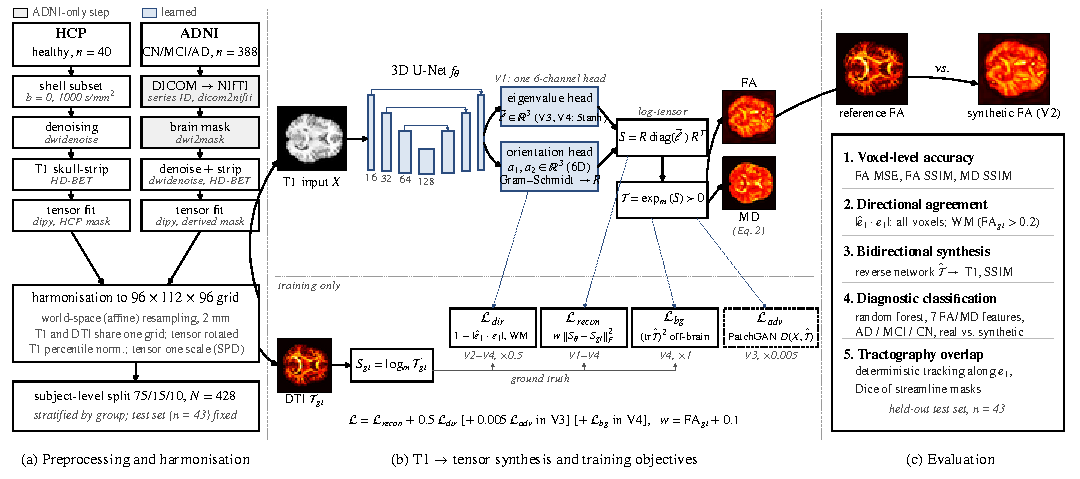
\includegraphics[width=\textwidth]{architecture_end_to_end.pdf}
\caption{End-to-end pipeline. (a) HCP and ADNI preprocessing (grey: ADNI-only steps) and world-space harmonization. (b) T1$\to$tensor synthesis: only the U-Net and its heads are learned (blue); the matrix exponential and the closed-form FA/MD equations are fixed mathematics, guaranteeing SPD output. Each loss box lists the variants that use it and its weight. (c) Evaluation on the held-out test set.}
\label{fig:pipeline}
\end{figure*}

\section{Methodology}
\label{sec:architecture}

\subsection{Pipeline Overview}
\label{sec:overview}
Let $X \in \mathbb{R}^{H \times W \times D}$ be a skull-stripped, intensity-normalized T1 volume, the only model input. Every variant computes
\begin{equation}
X \xrightarrow{\;f_\theta\;} S \xrightarrow{\;\exp_m\;} \mathcal{T} \xrightarrow{\;\text{Eq.~(2)}\;} (\text{FA},\,\text{MD}),
\label{eq:pipeline}
\end{equation}
where $f_\theta$ is a 3D U-Net producing a symmetric log-tensor $S(v)$ at each voxel $v$, $\exp_m$ is the matrix exponential mapping it to a diffusion tensor $\mathcal{T}(v)$, and FA/MD are computed analytically from the eigenvalues $\lambda_1\geq\lambda_2\geq\lambda_3$ of $\mathcal{T}$:
\begin{equation}
\text{MD} = \tfrac{\lambda_1+\lambda_2+\lambda_3}{3},\ \
\text{FA} = \sqrt{\tfrac{3}{2}\tfrac{\sum_i(\lambda_i-\text{MD})^2}{\sum_i\lambda_i^2}}.
\end{equation}
FA and MD are never predicted separately, so they stay consistent with the tensor field. The only learned step is $f_\theta$; the variants differ solely in how $f_\theta$ produces $S$ and in which loss terms shape it: V2 changes V1's output head and adds $\mathcal{L}_{dir}$, and V3 and V4 each add one further loss to V2 plus a $5\tanh$ eigenvalue bound (Fig.~\ref{fig:pipeline}b).

\subsection{Log-Euclidean Tensor Representation}
\label{sec:logeuclid}
A diffusion tensor must be SPD. Regressing tensor entries directly produces thousands of non-SPD voxels per volume \cite{paper1}, and post-hoc clipping of negative eigenvalues distorts tensor geometry. Following \cite{paper1}, each variant instead outputs six unconstrained values per voxel, assembled into a symmetric matrix $S(v)$ (the \emph{log-tensor}). Writing $S=U\,\mathrm{diag}(\mu)\,U^\top$,
\begin{equation}
\mathcal{T}(v)=\exp_m\!\big(S(v)\big)=U\,\mathrm{diag}\big(e^{\mu_1},e^{\mu_2},e^{\mu_3}\big)\,U^\top,
\end{equation}
and since $e^{\mu}>0$ for any real $\mu$, every possible network output is a valid SPD tensor. Ground-truth tensors are mapped into the same space by the inverse, $S_{gt}=\log_m(\mathcal{T}_{gt})$, with eigenvalues floored at $10^{-4}$ where preprocessing noise leaves them near zero or slightly negative. The shared reconstruction loss compares the two in log space,
\begin{equation}
\mathcal{L}_{recon} = \tfrac{1}{|V|}\textstyle\sum_v w(v)\,\|S_\theta(v)-S_{gt}(v)\|_F^2,\ \ w=\text{FA}_{gt}+0.1,
\label{eq:recon}
\end{equation}
i.e.\ the log-Euclidean distance, a proper metric on the SPD manifold, rather than an entry-wise distance between tensors. The weight $w$ gives white matter (high FA) proportionally more gradient without excluding other tissue.

\subsection{V1: Single-Head Baseline}
A 3D U-Net \cite{cicek2016} with three downsampling levels (channel widths 16--32--64, bottleneck 128), each block two $3^3$ convolutions with batch normalization and ReLU, max-pool downsampling, transposed-convolution upsampling, and skip concatenation ($\sim$1.4M parameters). A final $1^3$ convolution outputs the six log-tensor components, bounded by $5\tanh(\cdot)$ purely so that $\exp_m$ cannot overflow; SPD validity comes from $\exp_m$, not this bound. A single head produces all six components undifferentiated, with no distinction between tensor magnitude and orientation. V1 is trained with $\mathcal{L}_{recon}$ only.

\subsection{V2: Dual-Head Geometric Decoupling}
Predicting a tensor involves two problems of different difficulty: its \emph{magnitude} (three eigenvalues, a smooth, intensity-like quantity) and its \emph{orientation} (the eigenvector frame, a spatially coherent orientation field). V2 keeps V1's trunk but replaces the output layer with two $1^3$ convolutional heads (Fig.~\ref{fig:pipeline}b):

\textit{Eigenvalue head:} three unconstrained log-eigenvalues $\vec\ell$; overflow is prevented by capping eigenvalues at 20 inside $\exp_m$. V3 and V4 additionally bound them by $5\tanh(\cdot)$, as in V1.

\textit{Orientation head:} six values forming two 3-vectors $a_1,a_2$ (the continuous 6D rotation representation \cite{zhou2019continuity}), converted to a rotation matrix $R=[r_1\,r_2\,r_3]$ by Gram--Schmidt:
\begin{equation}
r_1=\tfrac{a_1}{\|a_1\|},\ \ r_2=\tfrac{a_2-(r_1^{\top}a_2)\,r_1}{\|a_2-(r_1^{\top}a_2)\,r_1\|},\ \ r_3=r_1\times r_2 .
\end{equation}
Unlike quaternions or Euler angles, this representation has no discontinuities, which otherwise hamper regression of rotations \cite{zhou2019continuity}. The heads are recombined as
\begin{equation}
S=R\,\mathrm{diag}(\vec\ell)\,R^\top \;\Rightarrow\; \mathcal{T}=\exp_m(S)=R\,\mathrm{diag}(e^{\vec\ell})\,R^\top ,
\end{equation}
so $R$ and $\vec\ell$ \emph{are} the tensor's eigendecomposition by construction, and no eigendecomposition is needed in the forward pass. Because $\exp$ is monotonic, the predicted principal direction $\hat e_1$ is simply the column of $R$ at $\arg\max_i \ell_i$, which enables a directional loss on white-matter voxels ($V_{wm}$: FA$_{gt}>0.2$):
\begin{equation}
\mathcal{L}_{dir}=\tfrac{1}{|V_{wm}|}\textstyle\sum_{v\in V_{wm}}\big(1-|\hat e_1(v)\cdot e_1(v)|\big),
\end{equation}
where the absolute value makes the loss invariant to eigenvector sign. V2's loss is $\mathcal{L}=\mathcal{L}_{recon}+0.5\,\mathcal{L}_{dir}$.

\subsection{V3: Adversarial Training}
V3 adds a conditional 3D PatchGAN discriminator \cite{isola2017pix2pix} to V2, judging $(X,\mathcal{T})$ pairs patch-wise, i.e.\ whether a tensor field is realistic \emph{for this T1}; adversarial training gave strong directional accuracy in prior work \cite{paper1}. LSGAN loss, one-sided label smoothing (0.9) and a halved discriminator learning rate counter discriminator dominance. $\mathcal{L}=\mathcal{L}_{recon}+0.5\,\mathcal{L}_{dir}+0.005\,\mathcal{L}_{adv}$.

\subsection{V4: Explicit Background Suppression}
V4 tests whether nonzero diffusion predicted outside the brain (\emph{background bleed}) can be suppressed directly and stably, without an adversarial game. Background voxels are those where ground truth shows no tissue, $V_{bg}=\{v:\text{MD}_{gt}(v)<0.01\}$ (in normalized units), and the predicted tensor's trace is penalized there:
\begin{equation}
\mathcal{L}_{bg}=\tfrac{1}{|V_{bg}|}\textstyle\sum_{v\in V_{bg}}\big(\mathrm{tr}\,\hat{\mathcal{T}}(v)\big)^2,\quad \mathrm{tr}\,\hat{\mathcal{T}}=3\,\widehat{\text{MD}},
\end{equation}
which directly penalizes predicted diffusivity where none exists. It is computed on the physical tensor $\hat{\mathcal{T}}=\exp_m(S_\theta)$, not on $S_\theta$: the correct background prediction is a large \emph{negative} log-eigenvalue (near-zero diffusivity), so penalizing log-space magnitude would instead pull predictions toward $\ell=0$, i.e.\ unit diffusivity. $\mathcal{L}=\mathcal{L}_{recon}+0.5\,\mathcal{L}_{dir}+\mathcal{L}_{bg}$.

\subsection{Training and Augmentation}
Training uses $64^3$-voxel patches (batch size 2) sampled from the canonical volume, Adam ($1\times10^{-4}$; discriminator $5\times10^{-5}$ for V3), max 100 epochs, early-stopping patience 12, and gradient clipping (max norm 1.0; 0.5 for V3). Weights are verified finite after each optimizer step and automatically reverted on failure.

Training patches are augmented on the fly. A left--right reflection (probability 0.5) is applied jointly to the T1 and the tensor field \emph{with} tensor reorientation, $\mathcal{T}'=F\mathcal{T}F$ with $F=\mathrm{diag}(-1,1,1)$, so that $D_{xy}$ and $D_{xz}$ change sign; reflecting the volume without reorienting the tensor would pair mirrored anatomy with un-mirrored fiber directions. T1 intensities additionally receive random gamma ($[0.7,1.5]$), a smooth bias field, contrast/brightness ($\pm$10\%) and Gaussian noise ($\sigma\le0.03$). AD training subjects are drawn 1.3 times per epoch to reduce class imbalance. Validation and test data are never augmented.

\subsection{Validation Checks}
A \textbf{bidirectional synthesis check} trains a smaller reverse network (tensor$\to$T1) and compares the reconstructed T1 to the original, testing whether the synthesized tensor retains subject-specific anatomy. A \textbf{diagnostic classification check} trains a random forest (200 trees, max depth 4) on a 7-dimensional feature vector (whole-brain and white-matter FA/MD mean and standard deviation, white-matter fraction) to distinguish AD/MCI/CN, once on ground-truth and once on each variant's synthetic features; it is a feasibility check, not a diagnostic evaluation. A \textbf{tractography overlap check} computes the Dice overlap of real and synthetic streamline masks from a simple deterministic tracker along the principal eigenvector.

\section{Results}
\label{sec:results}
V1, V2 and V4 were trained and evaluated with the pipeline above on the same 43 test subjects (8 AD, 16 MCI, 15 CN, 4 HCP). V1 and V2 trained for 100 epochs (best 91 and 98; $\sim$5.2h and $\sim$10h), V4 stopped early at epoch 37 (best 25), and all converged stably. V3 is discussed in Section~\ref{sec:correction}.

\begin{table}[t]
\centering
\footnotesize
\setlength{\tabcolsep}{2.6pt}
\caption{Voxel-level and directional accuracy (mean $\pm$ s.d., $n=43$). FA MSE, FA/MD SSIM and Cos.(all) are computed over the full canonical volume; Cos.(WM) restricts to FA$_{gt}>0.2$; 0.5 is chance.}
\label{tab:main_results}
\begin{tabular}{lccccc}
\toprule
\textbf{Var.} & \textbf{FA MSE} & \textbf{FA SSIM} & \textbf{MD SSIM} & \textbf{Cos.(all)} & \textbf{Cos.(WM)} \\
\midrule
V1 & .0092{\scriptsize$\pm$.0014} & .073{\scriptsize$\pm$.006} & .630{\scriptsize$\pm$.033} & .481 & .621{\scriptsize$\pm$.024} \\
V2 & \textbf{.0065}{\scriptsize$\pm$.0011} & \textbf{.152}{\scriptsize$\pm$.011} & \textbf{.842}{\scriptsize$\pm$.037} & .388 & \textbf{.802}{\scriptsize$\pm$.044} \\
V4 & .0083{\scriptsize$\pm$.0013} & .110{\scriptsize$\pm$.009} & .558{\scriptsize$\pm$.021} & \textbf{.923} & .716{\scriptsize$\pm$.034} \\
\bottomrule
\end{tabular}
\end{table}

V2 is the most accurate variant on every in-brain metric (Table~\ref{tab:main_results}). Cos.(all) is dominated by background voxels, where the ground-truth tensor is zero and has no defined direction; V4 scores highly there because it also predicts near-zero tensors, so this column reflects background behavior, not fiber direction.

\subsection{Ablation: Contribution of Each Component}
\label{sec:ablation}
Because each variant adds one component group to its predecessor, consecutive variants form an ablation; Table~\ref{tab:ablation} isolates the change each step produces, tested per subject with paired Wilcoxon signed-rank tests.

\begin{table}[t]
\centering
\footnotesize
\setlength{\tabcolsep}{2.0pt}
\caption{Ablation: change in each metric from adding one component group (paired, $n=43$). ``Improved'': subjects that improved on that metric. All changes: Wilcoxon $p<10^{-12}$.}
\label{tab:ablation}
\begin{tabular}{lcccc}
\toprule
\textbf{Step (component added)} & \textbf{FA MSE} & \textbf{FA SSIM} & \textbf{MD SSIM} & \textbf{Cos.(WM)} \\
\midrule
V1$\to$V2 (dual head, $\mathcal{L}_{dir}$) & $-0.0027$ & $+0.080$ & $+0.213$ & $+0.180$ \\
\quad improved & 43/43 & 43/43 & 43/43 & 43/43 \\
V2$\to$V4 ($\mathcal{L}_{bg}$, bounded $\vec\ell$) & $+0.0017$ & $-0.042$ & $-0.285$ & $-0.085$ \\
\quad improved & 0/43 & 0/43 & 0/43 & 0/43 \\
\bottomrule
\end{tabular}
\end{table}

\textit{Geometric decoupling (V1$\to$V2)} is the dominant component: white-matter cosine similarity rises from $0.621$ to $0.802$, MD SSIM from $0.630$ to $0.842$, FA SSIM doubles and FA MSE falls by 29\%. The improvement is not an average effect: \emph{every one} of the 43 test subjects improves on all four metrics (Fig.~\ref{fig:per_subject}). This step introduces the dual head and $\mathcal{L}_{dir}$ together, which are not separated here.

\textit{Explicit background suppression (V2$\to$V4)} lowers every in-brain metric --- MD SSIM by $0.285$, Cos.(WM) by $0.085$, FA SSIM by $0.042$ --- and raises FA MSE, again for all 43 subjects. With world-space harmonization, V2 shows no volume-wide background bleed, only a faint rim outside the brain (Fig.~\ref{fig:qualitative}), so $\mathcal{L}_{bg}$ has little to remove and acts mainly as a competing objective; V4's lower-contrast MD is consistent with the trace penalty pulling diffusivity down. This step also adds the $5\tanh$ eigenvalue bound; the two are not separated.

\begin{figure}[t]
\centering
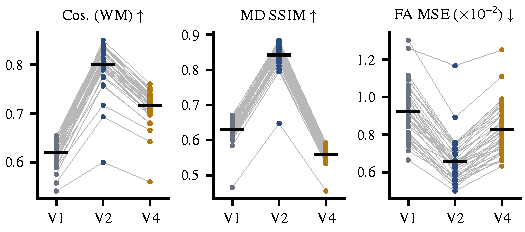
\includegraphics[width=0.92\linewidth]{fig_per_subject.pdf}
\caption{Per-subject results on the 43 test subjects; grey lines connect the same subject, black bars mark the mean. Every subject improves from V1 to V2 and worsens from V2 to V4. The low outlier in each panel is one CN subject whose T1 and diffusion brains overlap poorly even after harmonization.}
\label{fig:per_subject}
\end{figure}

\begin{figure}[t]
\centering
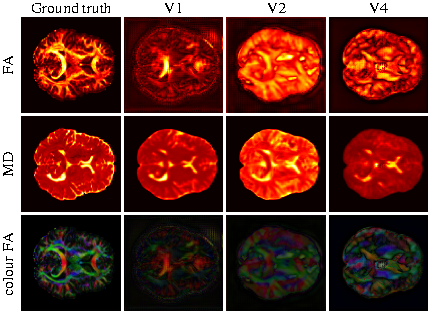
\includegraphics[width=0.8\linewidth]{fig_qualitative_comparison_v2.pdf}
\caption{Qualitative comparison, representative test subject (axial slice). Colour FA: red left--right, green anterior--posterior, blue inferior--superior. V2 reproduces MD structure closely and the dominant fiber orientations, but its FA is smooth and over-estimated in grey matter; fine high-FA tracts remain the main gap.}
\label{fig:qualitative}
\end{figure}

\subsection{Effect of Harmonization: Voxel-Size vs.\ World-Space Resampling}
\label{sec:correction}
We compare against a baseline pipeline that resamples each volume independently by its voxel spacing and centre-crops it, ignoring position and field of view --- a common simplification. Because ADNI T1 acquisitions cover a larger field of view (including the neck) than the diffusion series, this displaces the modalities relative to each other: the median T1/diffusion brain Dice is $0.79$--$0.82$ for the ADNI groups ($0.93$ for HCP, whose modalities share AC-PC space), and 56\% of the QC sample falls below $0.85$. World-space harmonization raises the ADNI medians to $0.91$--$0.92$ and leaves 3\% below $0.85$. The baseline pipeline also omits the site-006 gradient correction and applies left--right reflection without tensor reorientation.

Table~\ref{tab:correction} compares both pipelines on the same test subjects; the three differences are applied together, so their individual effects are not separated. Every evaluated variant improves on every metric under world-space harmonization, and the qualitative picture changes. Under the baseline pipeline V2 predicts diffusion across nearly the entire volume, and background suppression (V3 or V4) cuts FA MSE by $\sim$72\% at a cost in MD SSIM, which suggests an FA/MD trade-off. That artifact appears to stem largely from the misalignment --- the network learns to predict diffusion where the misaligned T1 shows no tissue --- and with aligned inputs the trade-off disappears. V3, which targets the same artifact, was therefore evaluated only under the baseline pipeline, where it never fully converged and matched V4 within $0.0002$ FA MSE.

\begin{table}[t]
\centering
\footnotesize
\setlength{\tabcolsep}{2.4pt}
\caption{Baseline (voxel-size) vs.\ world-space pipeline (baseline$\to$world-space), same 43 test subjects. $^\dagger$Baseline V1 was evaluated on a smaller 25-subject split.}
\label{tab:correction}
\begin{tabular}{lcccc}
\toprule
\textbf{Var.} & \textbf{FA MSE} & \textbf{MD SSIM} & \textbf{Cos.(WM)} & \textbf{Bidir.\ SSIM} \\
\midrule
V1$^\dagger$ & .0220$\to$.0092 & .518$\to$.630 & .510$\to$.621 & .050$\to$.236 \\
V2 & .0345$\to$.0065 & .735$\to$.842 & .613$\to$.802 & .142$\to$.262 \\
V3 & .0097$\to$\;--\; & .503$\to$\;--\; & .597$\to$\;--\; & .152$\to$\;--\; \\
V4 & .0099$\to$.0083 & .503$\to$.558 & .588$\to$.716 & .101$\to$.186 \\
\bottomrule
\end{tabular}
\end{table}

\subsection{Consistency Across Groups and Sites}
V2's accuracy is nearly identical across diagnostic groups and data sources: Cos.(WM) is $0.789$ (AD), $0.808$ (MCI), $0.803$ (CN) and $0.795$ (HCP), and MD SSIM $0.851$, $0.835$, $0.838$ and $0.872$. The four HCP subjects --- a different scanner, protocol and population, only 9\% of training data --- are on par with ADNI. The seven test subjects from ADNI site 006 reach $0.813$ versus $0.799$ for the remaining subjects, confirming the gradient correction.

\subsection{Downstream Checks and Comparison with Prior Work}
Bidirectional SSIM and tractography Dice are both highest for V2 (Table~\ref{tab:other_results}). In the classification check, random forests on real DTI features reach $0.462$ accuracy (macro-F1 $0.400$); synthetic features from V2 and V4 reach $0.436$ and $0.462$ (macro-F1 $0.446$, $0.454$), and V1 $0.333$. All are close to the majority-class baseline of $0.410$ (MCI) and the three-class chance level of $0.333$, so the experiment shows only that synthetic features carry roughly as much group information as real ones under this simple classifier; it is a feasibility check, not evidence of diagnostic performance.

\begin{table}[t]
\centering
\small
\setlength{\tabcolsep}{4pt}
\caption{Bidirectional synthesis, tractography overlap (Dice) and classification (39 ADNI test subjects; majority-class accuracy $0.410$).}
\label{tab:other_results}
\begin{tabular}{lcccc}
\toprule
\textbf{Variant} & \textbf{Bidir.\ SSIM} & \textbf{Tract.\ Dice} & \textbf{Acc.} & \textbf{Macro-F1} \\
\midrule
Real DTI & -- & -- & 0.462 & 0.400 \\
V1 & 0.236 & 0.147 & 0.333 & 0.349 \\
V2 & \textbf{0.262} & \textbf{0.193} & 0.436 & 0.446 \\
V4 & 0.186 & 0.164 & 0.462 & 0.454 \\
\bottomrule
\end{tabular}
\end{table}

Against the closest literature precedents, the like-for-like directional comparison is white-matter cosine similarity: $0.80$ here (V2) versus $0.86$ at FA~$\geq0.2$ for Anctil-Robitaille et al.\ \cite{paper1}, on a healthy, single-protocol cohort 2.5 times larger. Our FA SSIM is not directly comparable with published values (e.g.\ $0.86$ \cite{paper10}): it is computed per slice over the full volume, where background and prediction smoothness dominate.

\section{Discussion}
\label{sec:discussion}
\textit{Choosing a variant for an application.} With world-space harmonization there is no FA/MD trade-off to balance: V2 is best for every downstream use evaluated --- MD-based measures such as dementia markers, fiber direction and tractography, and FA statistics. Where background-free maps are needed (visual review, voxelwise statistics), V2's output should be masked post hoc with the T1 brain mask, at no cost to in-brain accuracy, rather than trained with $\mathcal{L}_{bg}$. If a future dataset shows volume-wide bleed, $\mathcal{L}_{bg}$'s weight should be tuned on validation data for the metric that matters to the intended use, since it costs MD structure first.

\textit{Dataset size and generalization.} With 43 test subjects, small group differences should not be over-interpreted, but the main effects are large relative to subject variability: every subject moves the same way at each ablation step. Performance is also consistent across diagnostic groups, data sources and the gradient-corrected ADNI site. The test subjects nevertheless come from the same two studies as the training data, so this is not external validation; an independent multi-site dataset is required before any claim of generalization to new scanners or clinics.

\textit{Interpretability.} Only the T1$\to$log-tensor network is learned; $\exp_m$ and the FA/MD equations are fixed, so every FA or MD value can be verified from the predicted tensor.

\section{Conclusion}
\label{sec:conclusion}
This work presents a controlled comparison of log-Euclidean, SPD-guaranteed architectures for T1-to-DTI synthesis on a mixed healthy and clinical cohort. Magnitude/orientation decoupling is the dominant component, improving every metric for every test subject. On 43 held-out subjects, the dual-head model (V2) reaches a white-matter directional cosine similarity of $0.80$ (baseline $0.62$), close to the $0.86$ reported on a healthy single-protocol cohort, together with MD SSIM $0.84$ and FA MSE $0.0065$. It also gives the highest bidirectional SSIM ($0.26$) and tractography Dice ($0.19$), performs consistently across AD, MCI, CN and HCP subjects, and its synthetic features carry similar group information to real DTI in a three-class feasibility check. Independent resampling of T1 and diffusion volumes misaligns them and produces artifacts that mimic an architectural trade-off; with world-space harmonization, explicit background suppression no longer helps, making cross-modal alignment a first-order concern for multi-modal synthesis.

\section{Limitations and Future Scope}
\label{sec:limitations}
Predicted FA is spatially smooth and misses high-FA tracts. The V1$\to$V2 step combines the dual head and $\mathcal{L}_{dir}$, and the V2$\to$V4 step combines $\mathcal{L}_{bg}$ with a $5\tanh$ eigenvalue bound; V4 stopped earlier than V2 under the same rule; V3 was evaluated only under the baseline pipeline; and the three pipeline differences were evaluated jointly. Harmonization relies on scanner affines rather than image registration, and one test subject retains poor T1/diffusion overlap. The test set is small and drawn from the training studies, tractography uses a coarse custom tracker, and classification is a feasibility check only. Future work: external multi-site validation before any diagnostic use; ablations separating the dual head from $\mathcal{L}_{dir}$ and the individual pipeline differences; better fine FA contrast through capacity, data and structure-aware losses; image-based T1-to-diffusion registration; and a validated probabilistic tractography pipeline with gradient-based saliency.

\begin{thebibliography}{12}

\bibitem{paper1}
B. Anctil-Robitaille et al., ``Manifold-aware synthesis of high-resolution diffusion from structural imaging,'' \textit{Frontiers in Neuroimaging}, vol. 1, 2022.

\bibitem{paper2}
T. Chattopadhyay et al., ``Generating diffusion MRI scalar maps from T1-weighted images using Reversible GANs,'' \textit{bioRxiv}, 2025.

\bibitem{paper3}
H. Tatekawa et al., ``Deep learning-based diffusion tensor image generation model: a proof-of-concept study,'' \textit{Scientific Reports}, vol. 14, 2024.

\bibitem{paper4}
T. Chattopadhyay et al., ``Synthetic diffusion tensor imaging maps generated by 2D and 3D probabilistic diffusion models,'' \textit{bioRxiv}, 2025.

\bibitem{paper5}
X. Zhu et al., ``When diffusion MRI meets diffusion model,'' in \textit{Proc. MICCAI}, 2024.

\bibitem{paper6}
Y. Chen et al., ``Improved dementia prediction in cerebral small vessel disease using deep learning--derived diffusion scalar maps from T1,'' \textit{Stroke}, vol. 55, pp. 2254--2263, 2024.

\bibitem{paper7}
X. Du, F. M. Cozzi, and R. Jena, ``Revolutionizing brain tumor imaging: generating synthetic 3D FA maps from T1-weighted MRI using CycleGAN models,'' \textit{arXiv:2505.03662}, 2025.

\bibitem{paper8}
X. Zhang et al., ``Structure-aware MRI translation: multi-modal latent diffusion model with arbitrary missing modalities,'' in \textit{Proc. MICCAI}. Springer, 2025, pp. 508--518.

\bibitem{paper9}
Y. Chen et al., ``Spherical harmonics-based deep learning achieves generalized and accurate diffusion tensor imaging,'' \textit{IEEE JBHI}, vol. 29, no. 1, pp. 456--467, 2025.

\bibitem{paper10}
S. Kim et al., ``Macro2Micro: a rapid and precise cross-modal MRI synthesis using multi-scale structural brain similarity,'' \textit{arXiv:2412.11277}, 2024.

\bibitem{cicek2016}
\"O. \c{C}i\c{c}ek et al., ``3D U-Net: learning dense volumetric segmentation from sparse annotation,'' in \textit{Proc. MICCAI}, 2016, pp. 424--432.

\bibitem{zhou2019continuity}
Y. Zhou et al., ``On the continuity of rotation representations in neural networks,'' in \textit{Proc. CVPR}, 2019, pp. 5745--5753.

\bibitem{isola2017pix2pix}
P. Isola et al., ``Image-to-image translation with conditional adversarial networks,'' in \textit{Proc. CVPR}, 2017, pp. 1125--1134.

\end{thebibliography}

\end{document}
